\documentclass[../TG_magistrsko_delo_sections.tex]{subfiles}
\graphicspath{{\subfix{../images/}}}

\begin{document}
V tem poglavju bomo spoznali topologijo urejenih prostorov in posebne urejene prostore s topologijo urejenih prostorov, ki jih imenujemo linearni kontinuum. Gre za neke vrste posplošitev premice realnih števil. Pokazali bomo, da je linearni kontinuum prostor Šarkovskega.

Naj bo množica $X$ urejena s strogo linearno relacijo $<$. Za dana elementa $a, b \in X$, za katera velja neenakost $a<b$, lahko definiramo štiri podmnožice prostora $X$, ki jih imenujemo intervali s krajišči $a$ in $b$. To so:
 %Na množici $X$ imamo dve vrsti odprtih množic, ki ju zapišemo na naslednji način:
\begin{equation*} %\label{eq1}
\begin{split}
(a, b) &= \{x \in X: a< x <b\} \\ 
(a, b] &= \{x \in X: a< x \leq b\} \\ 
[a, b) &= \{x \in X: a \leq x< b\} \\ 
[a, b] &= \{x \in X: a \leq x \leq b\}
\end{split}
\end{equation*}

\begin{opomba}\label{op:intervali}
Interval $(a, b)$ imenujemo odprti interval, intervalu $(a, b]$ rečemo pol odprti interval, interval $[a, b)$ je pol zaprti interval, interval $[a, b]$ pa je zaprti interval.
\end{opomba}

\begin{definicija}
Naj bo $X$ množica z vsaj dvema elementoma urejena z relacijo $<$ in naj bo $B$ družina množic, ki vsebuje intervale naslednjih tipov:
\begin{enumerate}
\item Vsi odprti intervali $(a, b) \in X$.
\item Vsi intervali $[a_0, b) \in X$, kjer je $a_0$ najmanjši element (če obstaja) množice $X$.
\item Vsi intervali $(a, b_0] \in X$, kjer je $b_0$ največji element (če obstaja) množice $X$.
\end{enumerate}
Družina množic $B$ je baza za topologijo na množici $X$, ki jo imenujemo topologija urejenih množic.
\end{definicija}

\begin{opomba}\label{op:ekstremi}
Če množica $X$ nima najmanjšega elementa, potem baza $B$ ne vsebuje intervalov tipa 2 in če množica $X$ nima največjega elementa, potem baza $B$ ne vsebuje intervalov tipa 3.
\end{opomba}

Prepričati se moramo, da zgoraj opisana družina množic $B$ res predstavlja bazo topologije na množici $X$ urejeni z linearno relacijo $<$. Družina podmnožic prostora $X$ je baza topologije na prostoru $X$, če sta izpolnjeni naslednji lastnosti:
\begin{enumerate}[label={(b\arabic*)}]
\item Množice iz družine $B$ pokrijejo celoten prostor $X$. Torej, vsaka točka $x \in X$ je vsebovana v neki množici $B_1 \in B$. \label{baza1}
\item Za vsaki množici $B_1, B_2 \in B$ in vsako točko $x\in B_1 \cap B_2$ obstaja množica $B_3 \in B$, za katero velja $x \in B_3 \subseteq B_1 \cap B_2$.\label{baza2}
\end{enumerate}
Preverimo najprej pogoj \ref{baza1}.
 Najprej moramo preveriti, da je vsaka točka množice $X$ vsebovana v nekem intervalu iz družine $B$. Če je točka $x$ enaka $a_0$, potem velja $x \in [a_0, a)$ za neko točko $a \in X$. Podobno lahko sklepamo v primeru, ko je $x = b_0$. Če je $x \neq a_0$ in $x \neq b_0$, potem zagotovo obstaja

\begin{definicija}
\emph{Linearni kontinuum} je linearno urejena množica $S$, ki ima naslednji lastnosti:
\begin{enumerate}
\item Vsaka navzgor omejena podmnožica $A \subseteq S$ ima najmanjšo zgornjo mejo v $S$,
\item za vsaki dve števili $x, y \in S$ obstaja število $z \in S$, za katerega je $x<z<y$.
\end{enumerate}
\end{definicija}

\begin{primer}
Enotski kvadrat $[0, 1] \times [0, 1]$ 
\end{primer}

\begin{figure}[h]
  \centering
  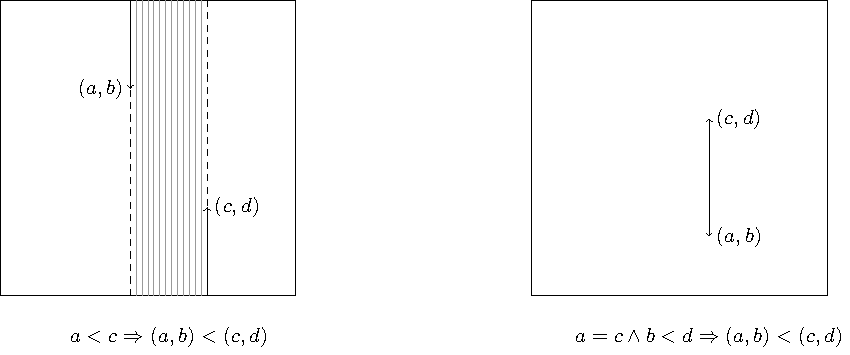
\includegraphics{urejen-kvadrat.pdf}
% \caption[caption za v kazalo]{Dolg caption pod sliko}
  \caption[Primer vektorske slike.]{Relacije pokritja v trditvi~\ref{trd:pokritja} lahko prikažemo z grafom.}
  \label{fig:varsavski_lok}
\end{figure}

\begin{trditev}
Strogo linearno urejena množica $X$ s topologijo urejenih množic je linearni kontinuum natanko tedaj, ko je povezana.
\end{trditev}
\begin{proof}
Predpostavimo, da je prostor $X$ s topologijo urejenih množic linearni kontinuum. Dokazali bomo, da je prostor $X$ povezan.  
\end{proof}

\begin{izrek}
Naj bo $f : X \to Y$ zvezna funkcija, kjer je $X$ povezan prostor in $Y$ urejen prostor s topologijo urejenih množic. Če sta $a$ in $b$ dve točki v prostoru $X$ in je $r$ točka v prostoru $Y$, ki leži med točkama $f(a)$ in $f(b)$, potem obstaja točka $c \in X$, da velja $f(c) = r$.
\end{izrek}
\begin{proof}
Privzemimo predpostavke izreka. Množici $=f(X) \cap (-\infty, r)$ in $B=f(X) \cap (r, \infty)$ sta disjunktni in neprazni, saj ena množica vsebuje točko $f(a)$, druga pa točko $f(b)$. Obe sta odprti v $f(X)$ saj smo ju dobili kot presek odprtega intervala z množico $f(X)$. Če ne obstaja taka točke $c \in X$, da je $f(c) = r$, potem je $f(X)$ unija množic $A$ in $B$. Na ta način smo dobili separacijo množice $f(X)$, kar pa je protislovje, saj je slika povezane množice z zvezno preslikavo povezana.
\end{proof}

\begin{lema}\label{lem:K}
Naj bo $L$ linearni kontinuum s topologijo urejenih množic. Naj bosta $I$ in $J$ zaprta intervala v $L$ in $f:L \to L$ zvezna funkcija. Če je $J \subseteq f(I)$, obstaja zaprt interval $K \subseteq I$, za katerega je $f(K) = J$.
\end{lema}
\begin{proof}
Izberemo taki točki $p, q \in I$, da velja $p<q$ in $J=[f(p), f(q)]$ ali $J=[f(q), f(p)]$. Definiramo točko $p \leq r < q$:
$$r= \sup\{x \in [p, q] : f(x) = f(p)\}.$$
Trdimo, da je $f(r) = f(p)$. V nasprotnem primeru obstaja odprta množica $V$, ki vsebuje točko $f(r)$ in ne vsebuje točke $f(p)$.To je res, ker je prostor $L$ Hausdorffov. Zaradi zveznosti funkcije $f$ obstaja taka odprta okolica $U$ točke $r$, da je $f(U) \subseteq V$. Ker je $L$ linearni kontinuum obstaja taka točka $p \leq r' < r$, za katero je interval $[r', r]$ vsebovan v množici $U$. Torej je $f([r', r]) \subseteq V$, kar pomeni, da $f(p) \notin f([r', r])$. To pa je protislovje z definicijo točke $r$ kot supremum množice.
Sedaj definiramo $r<s \leq q$:
$$r= \inf\{x \in [r, q] : f(x) = f(q)\}.$$ 
Enako kot prej se prepričamo, da je $f(s) = f(q)$. Zapišimo $Q = [r, s]$ in pokažimo, da je $f(Q) = J$. Izrek o vmesni vrednosti zagotavlja, da je interval $J$ vsebovan v množici $f([r, s])$. Velja tudi $f([r, s]) \subseteq J$, saj v nasprotnem primeru obstaja $r<x<s$, za katerega velja $f(x) \notin J$. Če je $f(x) < f(p) < f(q)$ ali $f(q) < f(p) < f(x)$, potem po izreku o vmesni vrednosti obstaja tak $x'$, da velja $r<x<x'<s$ in $f(p) = f(x')$. to pa je protislovje z definicijo točke $r$ kot supremum. Če je $f(x) < f(q) < f(p)$ ali $f(p) < f(q) < f(x)$, to privede do protislovja z definicijo točke $s$ kot infimum. To pomeni, da res velja $J = f(Q)$.
\end{proof}

\begin{lema}
Naj bo $L$ linearni kontinuum v topologiji urejenih množic. Naj bosta $I$ zaprt interval v $L$ in $f:L \to L$ zvezna funkcija. Če je $I \subseteq f(I)$, potem ima $f$ negibno točko $x \in I$.
\end{lema}
\begin{proof}
S pomočjo leme~\ref{lem:K} ugotovimo, da obstaja zaprt interval $Q \subseteq I$, za katerega je $f(Q) = I$. Pokazali bomo, da ima funkcija $f$ negibno točko v intervalu $Q$. Predpostavimo, da funkcija $f$ na intervalu $Q$ nima negibne točke. Potem lahko zapišemo $Q = A \cup B$, kjer je:
\begin{equation*} %\label{eq1}
\begin{split}
A &= \{x \in L : x < f(x)\}, \\ 
B &= \{x \in L : x > f(x)\}.
\end{split}
\end{equation*}
Trdimo, da je množica $A$ odprta. Za vsako točko $x \in A$ lahko izberemo točko $z \in (x, f(x))$ in odprto okolico $U \subseteq  (-\infty, z)$ točke $x$, za katero velja $f(U) \subseteq (z, \infty)$. Ker je množica $U$ podmnožica množoce $A$, je točka $x$ notranja točka množice $A$. Množica $A$ je odprta. Podobno lahko dokažemo, da je množica $B$ odprta. Množici $Q \cap A$ in $Q \cap B$ sta odprti podmnožici množice $Q$ za kateri velja $Q = (Q \cap A) \cup (Q \cap B)$. Radi bi videli, da sta množici $Q \cap A$ in $Q \cap B$ neprazni. Zapišimo $I = [c, d]$. Ker je $f(Q) = I$, obstaja $x' \in Q$, za katerega je $f(x') =d$. Ker $f$ nima fiksne točke na $Q$, je $x' \neq d$. Interval $Q$ je pomnožica intervala $I$, zato velja $x' < f(x') = d$, kar pomeni, da je $x' \in Q \cap A$. Analogno poiščemo točko $x'' \in Q - \{c\}$ z lastnostjo: $f(x'') = c$ in $x'' \in Q \cap B$. Torej, množici $Q \cap A$ in $Q \cap B$ tvorita separacijo povezanega prostora $Q$, kar je protislovje. Funkcija $f$ ima negibno točko v intervalu $Q$.
\end{proof}

\end{document}